\section{Python 数据结构的性能}
        
现在你对大 O 算法和不同函数之间的差异有了了解。本节的目标是告诉你 Python 列表和字典操作的 大O 性能。然后我们将做一些基于时间的实验来说明每个数据结构的花销和使用这些数据结构的好处。重要的是了解这些数据结构的效率,因为它们是本书实现其他数据结构所用到的基础模块。本节中,我们将不会说明为什么是这个性能。在后面的章节中,你将看到列表和字典一些可能的实现,以及性能是如何取决于实现的。


\subsection{列表}
        
Python 的设计者在实现列表数据结构的时候有很多选择。每一个这种选择都可能影响列表操作的性能。为了帮助他们做出正确的选择,他们查看了最常使用列表数据结构的方式,并且优化了实现,以便使得最常见的操作非常快。当然,他们还试图使较不常见的操作快速,但是当需要做出折衷时,较不常见的操作的性能通常牺牲以支持更常见的操作。

两个常见的操作是索引和分配到索引位置。无论列表有多大,这两个操作都需要相同的时间。当这样的操作和列表的大小无关时,它们是 $O(1)$。
另一个非常常见的编程任务是增加一个列表。有两种方法可以创建更长的列表,可以使用 append 方法或拼接运算符。append 方法是 $O(1)$。 然而,拼接运算符是 $O(k)$,其中 $k$ 是要拼接的列表的大小。这对你来说很重要,因为它可以帮助你通过选择合适的工具来提高你自己的程序的效率。

让我们看看四种不同的方式,我们可以生成一个从0开始的n个数字的列表。首先,我们将尝试一个 for 循环并通过创建列表,然后我们将使用 append 而不是拼接。接下来,我们使用列表生成器创建列表,最后,也是最明显的方式,通过调用列表构造函数包装 range 函数。 

\lstinputlisting{code/list_compare.py}


要捕获我们的每个函数执行所需的时间,我们将使用 Python 的 timeit 模块。
timeit 模块旨在允许 Python 开发人员通过在一致的环境中运行函数并使用尽可能相似的操作系统的时序机制来进行跨平台时序测量。
要使用 timeit,你需要创建一个 Timer 对象,其参数是两个 Python 语句。
第一个参数是一个你想要执行时间的 Python 语句; 
第二个参数是一个将运行一次以设置测试的语句。
然后 timeit 模块将计算执行语句所需的时间。
默认情况下,timeit 将尝试运行语句一百万次。 
当它完成时,它返回时间作为表示总秒数的浮点值。
由于它执行语句一百万次,可以读取结果作为执行测试一次的微秒数。你还可以传递 timeit 一个参数名字为 number,允许你指定执行测试语句的次数。以下显示了运行我们的每个测试功能 1000 次需要多长时间。
\begin{lstlisting}
t1 = Timer("test1()", "from __main__ import test1")
print("concat ",t1.timeit(number=1000), "milliseconds")
t2 = Timer("test2()", "from __main__ import test2")
print("append ",t2.timeit(number=1000), "milliseconds")
t3 = Timer("test3()", "from __main__ import test3")
print("comprehension ",t3.timeit(number=1000), "milliseconds")
t4 = Timer("test4()", "from __main__ import test4")
print("list range ",t4.timeit(number=1000), "milliseconds")
\end{lstlisting}

\begin{lstlisting}[frame=no]
concat  6.54352807999 milliseconds
append  0.306292057037 milliseconds
comprehension  0.147661924362 milliseconds
list range  0.0655000209808 milliseconds
\end{lstlisting}
在上面的例子中,我们对 \lstinline|test1(), test2()| 等的函数调用计时,setup 语句可能看起来很奇怪,所以我们详细说明下。你可能非常熟悉 from ,import 语句,但这通常用在 python 程序文件的开头。在这种情况下,\lstinline|from __main__ import test1| 从 \lstinline|__main__| 命名空间导入到 timeit 设置的命名空间中。timeit 这么做是因为它想在一个干净的环境中做测试,而不会因为可能有你创建的任何杂变量,以一种不可预见的方式干扰你函数的性能。
从上面的试验清楚的看出,append 操作比拼接快得多。其他两种方法,列表生成器的速度是 append 的两倍。
最后一点,你上面看到的时间都是包括实际调用函数的一些开销,但我们可以假设函数调用开销在四种情况下是相同的,所以我们仍然得到的是有意义的比较。因此,拼接字符串操作需要 6.54 毫秒并不准确,而是拼接字符串这个函数需要 6.54 毫秒。你可以测试调用空函数所需要的时间,并从上面的数字中减去它。
现在我们已经看到了如何具体测试性能,见 Table2, 你可能想知道 pop 两个不同的时间。当列表末尾调用 pop 时,它需要 O(1), 但是当在列表中第一个元素或者中间任何地方调用 pop, 它是 O(n)。原因在于 Python 实现列表的方式,当一个项从列表前面取出,列表中的其他元素靠近起始位置移动一个位置。你会看到索引操作为 O(1)。python的实现者会权衡选择一个好的方案。

\begin{table}[htbp]
\centering
\begin{tabular}{ll} \hline
操作&大 O 效率 \\\hline
\lstinline|index[]|         & $O(1)$ \\
\lstinline|index assignment|& $O(1)$ \\
\lstinline|append|          & $O(1)$ \\
\lstinline|pop()|           & $O(1)$ \\
\lstinline|pop(i)|          & $O(n)$ \\
\lstinline|insert(i,item)|  & $O(n)$ \\
\lstinline|del|             & $O(n)$ \\
\lstinline|iteration|       & $O(n)$ \\
\lstinline|contains(in)|    & $O(n)$ \\
\lstinline|get slice [x:y]| & $O(k)$ \\
\lstinline|del slice|       & $O(n)$ \\
\lstinline|set slice|       & $O(n+k)$ \\
\lstinline|reverse|         & $O(n)$ \\
\lstinline|concatenate|     & $O(k)$ \\
\lstinline|sort|            & $O(n\log n)$ \\
\lstinline|multiply|        & $O(nk)$ \\\hline 
\end{tabular}
\end{table}


作为一种演示性能差异的方法,我们用 \lstinline|timeit| 来做一个实验。我们的目标是验证从列表从末尾 pop 元素和从开始 pop 元素的性能。同样,我们也想测量不同列表大小对这个时间的影响。我们期望看到的是,从列表末尾处弹出所需时间将保持不变,即使列表不断增长。而从列表开始处弹出元素时间将随列表增长而增加。

Listing 4 展示了两种 pop 方式的比较。从第一个示例看出,从末尾弹出需要 0.0003 毫秒。从开始弹出要花费 4.82 毫秒。对于一个 200 万的元素列表,相差 16000 倍。

需要注意的几点,第一, \lstinline|from __main__ import x| , 虽然我们没有定义一个函数,我们确实希望能够在我们的测试中使用列表对象 x, 这种方法允许我们只计算单个弹出语句,获得该操作最精确的测量时间。因为 timer 重复了 1000 次,该列表每次循环大小都减 1。但是由于初始列表大小为 200万,我们只减少总体大小的 0.05\%。
\begin{lstlisting}
popzero = timeit.Timer("x.pop(0)",
"from __main__ import x")
popend = timeit.Timer("x.pop()",
"from __main__ import x")

x = list(range(2000000))
popzero.timeit(number=1000)
4.8213560581207275

x = list(range(2000000))
popend.timeit(number=1000)
0.0003161430358886719
\end{lstlisting}
Listing 4
虽然我们第一个测试显示 \lstinline|pop(0)| 比 \lstinline|pop()| 慢, 但它没有证明 \lstinline|pop(0)| 是 $O(n)$, \lstinline|pop()|是 $O(1)$。要验证它,我们需要看下一系列列表大小的调用效果。
\begin{lstlisting}
popzero = Timer("x.pop(0)",
"from __main__ import x")
popend = Timer("x.pop()",
"from __main__ import x")
print("pop(0)   pop()")
for i in range(1000000,100000001,1000000):
x = list(range(i))
pt = popend.timeit(number=1000)
x = list(range(i))
pz = popzero.timeit(number=1000)
print("%15.5f, %15.5f" %(pz,pt))
\end{lstlisting}
Figure 3 展示了我们实验的结果,你可以看到,随着列表变长,pop(0) 时间也增加,而 pop() 时间保持非常平坦。这正是我们期望看到的 O(n)和 O(1)

\begin{figure}
\centering
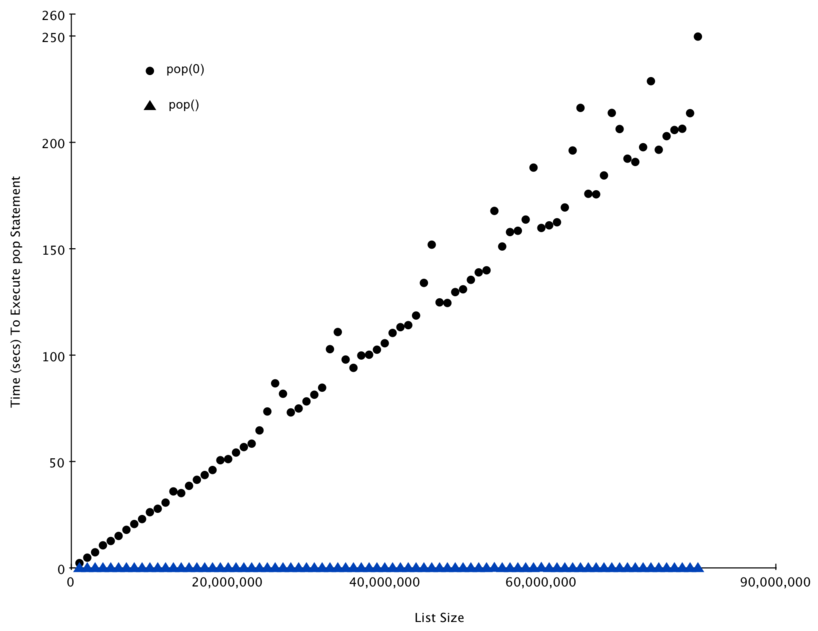
\includegraphics[width=5in]{images/poptime.png}
\end{figure}


\subsection{字典}

python 中第二个主要的数据结构是字典。你可能记得,字典和列表不同,你可以通过键而不是位置来访问字典中的项目。在本书的后面,你会看到有很多方法来实现字典。字典的 get 和 set 操作都是 O(1)。另一个重要的操作是 contains,检查一个键是否在字典中也是 O(1)。所有字典操作的效率总结在 Table3 中。关于字典性能的一个重要方面是,我们在表中提供的效率是针对平均性能。 在一些罕见的情况下,contains,get item 和 set item 操作可以退化为 O(n)。我们将在后面的章节介绍。
\begin{table}[htbp]
        \centering
        \begin{tabular}{ll} \hline
                操作&大 O 效率 \\\hline
                \lstinline|copy|         & $O(n)$ \\
                \lstinline|get item     |& $O(1)$ \\
                \lstinline|set item|     & $O(1)$ \\
                \lstinline|delete item|  & $O(1)$ \\
                \lstinline|contains(in)| & $O(1)$ \\
                \lstinline|iteration|    & $O(n)$  \\\hline 
        \end{tabular}
\end{table}

我们会在最后的实验中,将比较列表和字典之间的 contains 操作的性能。在此过程中,我们将确认列表的 contains 操作符是 O(n),字典的 contains 操作符是 O(1)。我们将在实验中列出一系列数字。然后随机选择数字,并检查数字是否在列表中。如果我们的性能表是正确的,列表越大,确定列表中是否包含任意一个数字应该花费的时间越长。
Listing 6 实现了这个比较。注意,我们对容器中的数字执行完全相同的操作。区别在于在第 7 行上 x 是一个列表,第9行上的 x 是一个字典。

\lstinputlisting{code/dict_time.py}

Figure 4 展示了 Listing6 的结果。你可以看到字典一直更快。 对于最小的列表大小为10,000个元素,字典是列表的89.4倍。对于最大的列表大小为990,000 个元素。字典是列表的11,603倍!你还可以看到列表上的contains运算符所花费的时间与列表的大小成线性增长。这验证了列表上的contains运算符是 O(n) 的断言。还可以看出,字典中的 contains 运算符的时间是恒定的,即使字典大小不断增长。事实上,对于字典大小为10,000个元素,contains操作占用0.004毫秒,对于字典大小为990,000个元素,它也占用0.004毫秒。
 

\begin{figure}
        \centering
        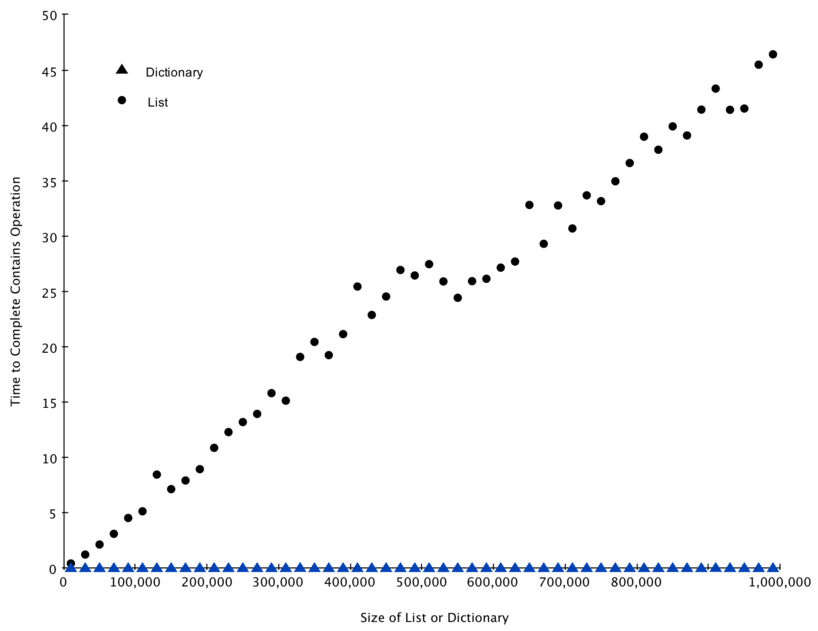
\includegraphics[width=5in]{images/dict_figure.png}
\end{figure}
由于 Python 是一种不断发展的语言,底层总是有变化的。 有关 Python 数据结构性能的最新信息可以在 Python 网站上找到。  
